\documentclass{article}

\usepackage{booktabs}
\usepackage{fancyhdr}
\usepackage{float}
\usepackage{graphicx}
\usepackage{helvet}
\usepackage{hyperref}
\usepackage{tabularx}
\usepackage{xcolor}

\usepackage{listings}

\lstset{frame=tblr,
  rulecolor=\color{lightgray},
  language=Java,
  aboveskip=5mm,
  belowskip=5mm,
  showstringspaces=false,
  columns=flexible,
  basicstyle={\small\ttfamily},
  numbers=none,
  % numberstyle=\tiny\color{gray},
  % keywordstyle=\color{blue},
  % commentstyle=\color{dkgreen},
  % stringstyle=\color{mauve},
  breaklines=true,
  breakatwhitespace=true,
  tabsize=3
}

\usepackage{framed}     % These needed for the code formatter
\usepackage{color}
\usepackage{fancyvrb}

% Use helvetica (sans) by default
\renewcommand{\familydefault}{\sfdefault}

% Greenish links
\hypersetup{
  colorlinks=true,
  linkcolor=blue!50!red,
  urlcolor=blue!50!red
}

\newcommand{\two}{\raise0.5ex\hbox{\footnotesize{2}}}

\newcommand{\iic}{I\two{}C}
\newcommand{\iicdriver}{I\two{}CDriver}

\setlength{\headheight}{40pt}
\setlength{\headsep}{0.2in}

\pagestyle{fancy}
\lhead{
\includegraphics[width=0.2\textwidth]{img/logo}}
\chead{\iicdriver{} User Guide}
\rhead{\thepage}
\cfoot{\textcopyright \the\year \ \ Excamera Labs}
\renewcommand{\headrulewidth}{0.5pt}
\renewcommand{\footrulewidth}{0.5pt}

\usepackage{array}
\newcolumntype{L}[1]{>{\raggedright\let\newline\\\arraybackslash\hspace{0pt}}m{#1}}
\newcolumntype{C}[1]{>{\centering\let\newline\\\arraybackslash\hspace{0pt}}m{#1}}
\newcolumntype{R}[1]{>{\raggedleft\let\newline\\\arraybackslash\hspace{0pt}}m{#1}}

\usepackage{setspace}

\newcommand{\heavyline}{\specialrule{1pt}{1pt}{1pt}}
\newcommand{\png}[1]{
\begin{figure}[H]
\begin{center}
\includegraphics[width=0.75\textwidth]{#1}
\end{center}
\end{figure}
}
\newcommand{\pngw}[2]{
\begin{figure}[H]
\begin{center}
\includegraphics[width=#2\textwidth]{#1}
\end{center}
\end{figure}
}

\newcommand{\mach}[1]{\texttt{\textbf{#1}}}
\newcommand{\gap}{\vspace{10pt}}


\makeatletter
\def\PY@reset{\let\PY@it=\relax \let\PY@bf=\relax%
    \let\PY@ul=\relax \let\PY@tc=\relax%
    \let\PY@bc=\relax \let\PY@ff=\relax}
\def\PY@tok#1{\csname PY@tok@#1\endcsname}
\def\PY@toks#1+{\ifx\relax#1\empty\else%
    \PY@tok{#1}\expandafter\PY@toks\fi}
\def\PY@do#1{\PY@bc{\PY@tc{\PY@ul{%
    \PY@it{\PY@bf{\PY@ff{#1}}}}}}}
\def\PY#1#2{\PY@reset\PY@toks#1+\relax+\PY@do{#2}}

\expandafter\def\csname PY@tok@gd\endcsname{\def\PY@tc##1{\textcolor[rgb]{0.63,0.00,0.00}{##1}}}
\expandafter\def\csname PY@tok@gu\endcsname{\let\PY@bf=\textbf\def\PY@tc##1{\textcolor[rgb]{0.50,0.00,0.50}{##1}}}
\expandafter\def\csname PY@tok@gt\endcsname{\def\PY@tc##1{\textcolor[rgb]{0.00,0.27,0.87}{##1}}}
\expandafter\def\csname PY@tok@gs\endcsname{\let\PY@bf=\textbf}
\expandafter\def\csname PY@tok@gr\endcsname{\def\PY@tc##1{\textcolor[rgb]{1.00,0.00,0.00}{##1}}}
\expandafter\def\csname PY@tok@cm\endcsname{\let\PY@it=\textit\def\PY@tc##1{\textcolor[rgb]{0.25,0.50,0.50}{##1}}}
\expandafter\def\csname PY@tok@vg\endcsname{\def\PY@tc##1{\textcolor[rgb]{0.10,0.09,0.49}{##1}}}
\expandafter\def\csname PY@tok@m\endcsname{\def\PY@tc##1{\textcolor[rgb]{0.40,0.40,0.40}{##1}}}
\expandafter\def\csname PY@tok@mh\endcsname{\def\PY@tc##1{\textcolor[rgb]{0.40,0.40,0.40}{##1}}}
\expandafter\def\csname PY@tok@go\endcsname{\def\PY@tc##1{\textcolor[rgb]{0.53,0.53,0.53}{##1}}}
\expandafter\def\csname PY@tok@ge\endcsname{\let\PY@it=\textit}
\expandafter\def\csname PY@tok@vc\endcsname{\def\PY@tc##1{\textcolor[rgb]{0.10,0.09,0.49}{##1}}}
\expandafter\def\csname PY@tok@il\endcsname{\def\PY@tc##1{\textcolor[rgb]{0.40,0.40,0.40}{##1}}}
\expandafter\def\csname PY@tok@cs\endcsname{\let\PY@it=\textit\def\PY@tc##1{\textcolor[rgb]{0.25,0.50,0.50}{##1}}}
\expandafter\def\csname PY@tok@cp\endcsname{\def\PY@tc##1{\textcolor[rgb]{0.74,0.48,0.00}{##1}}}
\expandafter\def\csname PY@tok@gi\endcsname{\def\PY@tc##1{\textcolor[rgb]{0.00,0.63,0.00}{##1}}}
\expandafter\def\csname PY@tok@gh\endcsname{\let\PY@bf=\textbf\def\PY@tc##1{\textcolor[rgb]{0.00,0.00,0.50}{##1}}}
\expandafter\def\csname PY@tok@ni\endcsname{\let\PY@bf=\textbf\def\PY@tc##1{\textcolor[rgb]{0.60,0.60,0.60}{##1}}}
\expandafter\def\csname PY@tok@nl\endcsname{\def\PY@tc##1{\textcolor[rgb]{0.63,0.63,0.00}{##1}}}
\expandafter\def\csname PY@tok@nn\endcsname{\let\PY@bf=\textbf\def\PY@tc##1{\textcolor[rgb]{0.00,0.00,1.00}{##1}}}
\expandafter\def\csname PY@tok@no\endcsname{\def\PY@tc##1{\textcolor[rgb]{0.53,0.00,0.00}{##1}}}
\expandafter\def\csname PY@tok@na\endcsname{\def\PY@tc##1{\textcolor[rgb]{0.49,0.56,0.16}{##1}}}
\expandafter\def\csname PY@tok@nb\endcsname{\def\PY@tc##1{\textcolor[rgb]{0.00,0.50,0.00}{##1}}}
\expandafter\def\csname PY@tok@nc\endcsname{\let\PY@bf=\textbf\def\PY@tc##1{\textcolor[rgb]{0.00,0.00,1.00}{##1}}}
\expandafter\def\csname PY@tok@nd\endcsname{\def\PY@tc##1{\textcolor[rgb]{0.67,0.13,1.00}{##1}}}
\expandafter\def\csname PY@tok@ne\endcsname{\let\PY@bf=\textbf\def\PY@tc##1{\textcolor[rgb]{0.82,0.25,0.23}{##1}}}
\expandafter\def\csname PY@tok@nf\endcsname{\def\PY@tc##1{\textcolor[rgb]{0.00,0.00,1.00}{##1}}}
\expandafter\def\csname PY@tok@si\endcsname{\let\PY@bf=\textbf\def\PY@tc##1{\textcolor[rgb]{0.73,0.40,0.53}{##1}}}
\expandafter\def\csname PY@tok@s2\endcsname{\def\PY@tc##1{\textcolor[rgb]{0.73,0.13,0.13}{##1}}}
\expandafter\def\csname PY@tok@vi\endcsname{\def\PY@tc##1{\textcolor[rgb]{0.10,0.09,0.49}{##1}}}
\expandafter\def\csname PY@tok@nt\endcsname{\let\PY@bf=\textbf\def\PY@tc##1{\textcolor[rgb]{0.00,0.50,0.00}{##1}}}
\expandafter\def\csname PY@tok@nv\endcsname{\def\PY@tc##1{\textcolor[rgb]{0.10,0.09,0.49}{##1}}}
\expandafter\def\csname PY@tok@s1\endcsname{\def\PY@tc##1{\textcolor[rgb]{0.73,0.13,0.13}{##1}}}
\expandafter\def\csname PY@tok@sh\endcsname{\def\PY@tc##1{\textcolor[rgb]{0.73,0.13,0.13}{##1}}}
\expandafter\def\csname PY@tok@sc\endcsname{\def\PY@tc##1{\textcolor[rgb]{0.73,0.13,0.13}{##1}}}
\expandafter\def\csname PY@tok@sx\endcsname{\def\PY@tc##1{\textcolor[rgb]{0.00,0.50,0.00}{##1}}}
\expandafter\def\csname PY@tok@bp\endcsname{\def\PY@tc##1{\textcolor[rgb]{0.00,0.50,0.00}{##1}}}
\expandafter\def\csname PY@tok@c1\endcsname{\let\PY@it=\textit\def\PY@tc##1{\textcolor[rgb]{0.25,0.50,0.50}{##1}}}
\expandafter\def\csname PY@tok@kc\endcsname{\let\PY@bf=\textbf\def\PY@tc##1{\textcolor[rgb]{0.00,0.50,0.00}{##1}}}
\expandafter\def\csname PY@tok@c\endcsname{\let\PY@it=\textit\def\PY@tc##1{\textcolor[rgb]{0.25,0.50,0.50}{##1}}}
\expandafter\def\csname PY@tok@mf\endcsname{\def\PY@tc##1{\textcolor[rgb]{0.40,0.40,0.40}{##1}}}
\expandafter\def\csname PY@tok@err\endcsname{\def\PY@bc##1{\setlength{\fboxsep}{0pt}\fcolorbox[rgb]{1.00,0.00,0.00}{1,1,1}{\strut ##1}}}
\expandafter\def\csname PY@tok@kd\endcsname{\let\PY@bf=\textbf\def\PY@tc##1{\textcolor[rgb]{0.00,0.50,0.00}{##1}}}
\expandafter\def\csname PY@tok@ss\endcsname{\def\PY@tc##1{\textcolor[rgb]{0.10,0.09,0.49}{##1}}}
\expandafter\def\csname PY@tok@sr\endcsname{\def\PY@tc##1{\textcolor[rgb]{0.73,0.40,0.53}{##1}}}
\expandafter\def\csname PY@tok@mo\endcsname{\def\PY@tc##1{\textcolor[rgb]{0.40,0.40,0.40}{##1}}}
\expandafter\def\csname PY@tok@kn\endcsname{\let\PY@bf=\textbf\def\PY@tc##1{\textcolor[rgb]{0.00,0.50,0.00}{##1}}}
\expandafter\def\csname PY@tok@mi\endcsname{\def\PY@tc##1{\textcolor[rgb]{0.40,0.40,0.40}{##1}}}
\expandafter\def\csname PY@tok@gp\endcsname{\let\PY@bf=\textbf\def\PY@tc##1{\textcolor[rgb]{0.00,0.00,0.50}{##1}}}
\expandafter\def\csname PY@tok@o\endcsname{\def\PY@tc##1{\textcolor[rgb]{0.40,0.40,0.40}{##1}}}
\expandafter\def\csname PY@tok@kr\endcsname{\let\PY@bf=\textbf\def\PY@tc##1{\textcolor[rgb]{0.00,0.50,0.00}{##1}}}
\expandafter\def\csname PY@tok@s\endcsname{\def\PY@tc##1{\textcolor[rgb]{0.73,0.13,0.13}{##1}}}
\expandafter\def\csname PY@tok@kp\endcsname{\def\PY@tc##1{\textcolor[rgb]{0.00,0.50,0.00}{##1}}}
\expandafter\def\csname PY@tok@w\endcsname{\def\PY@tc##1{\textcolor[rgb]{0.73,0.73,0.73}{##1}}}
\expandafter\def\csname PY@tok@kt\endcsname{\def\PY@tc##1{\textcolor[rgb]{0.69,0.00,0.25}{##1}}}
\expandafter\def\csname PY@tok@ow\endcsname{\let\PY@bf=\textbf\def\PY@tc##1{\textcolor[rgb]{0.67,0.13,1.00}{##1}}}
\expandafter\def\csname PY@tok@sb\endcsname{\def\PY@tc##1{\textcolor[rgb]{0.73,0.13,0.13}{##1}}}
\expandafter\def\csname PY@tok@k\endcsname{\let\PY@bf=\textbf\def\PY@tc##1{\textcolor[rgb]{0.00,0.50,0.00}{##1}}}
\expandafter\def\csname PY@tok@se\endcsname{\let\PY@bf=\textbf\def\PY@tc##1{\textcolor[rgb]{0.73,0.40,0.13}{##1}}}
\expandafter\def\csname PY@tok@sd\endcsname{\let\PY@it=\textit\def\PY@tc##1{\textcolor[rgb]{0.73,0.13,0.13}{##1}}}

\def\PYZbs{\char`\\}
\def\PYZus{\char`\_}
\def\PYZob{\char`\{}
\def\PYZcb{\char`\}}
\def\PYZca{\char`\^}
\def\PYZam{\char`\&}
\def\PYZlt{\char`\<}
\def\PYZgt{\char`\>}
\def\PYZsh{\char`\#}
\def\PYZpc{\char`\%}
\def\PYZdl{\char`\$}
\def\PYZhy{\char`\-}
\def\PYZsq{\char`\'}
\def\PYZdq{\char`\"}
\def\PYZti{\char`\~}
% for compatibility with earlier versions
\def\PYZat{@}
\def\PYZlb{[}
\def\PYZrb{]}
\makeatother



\begin{document}

\newpage
\begin{center}
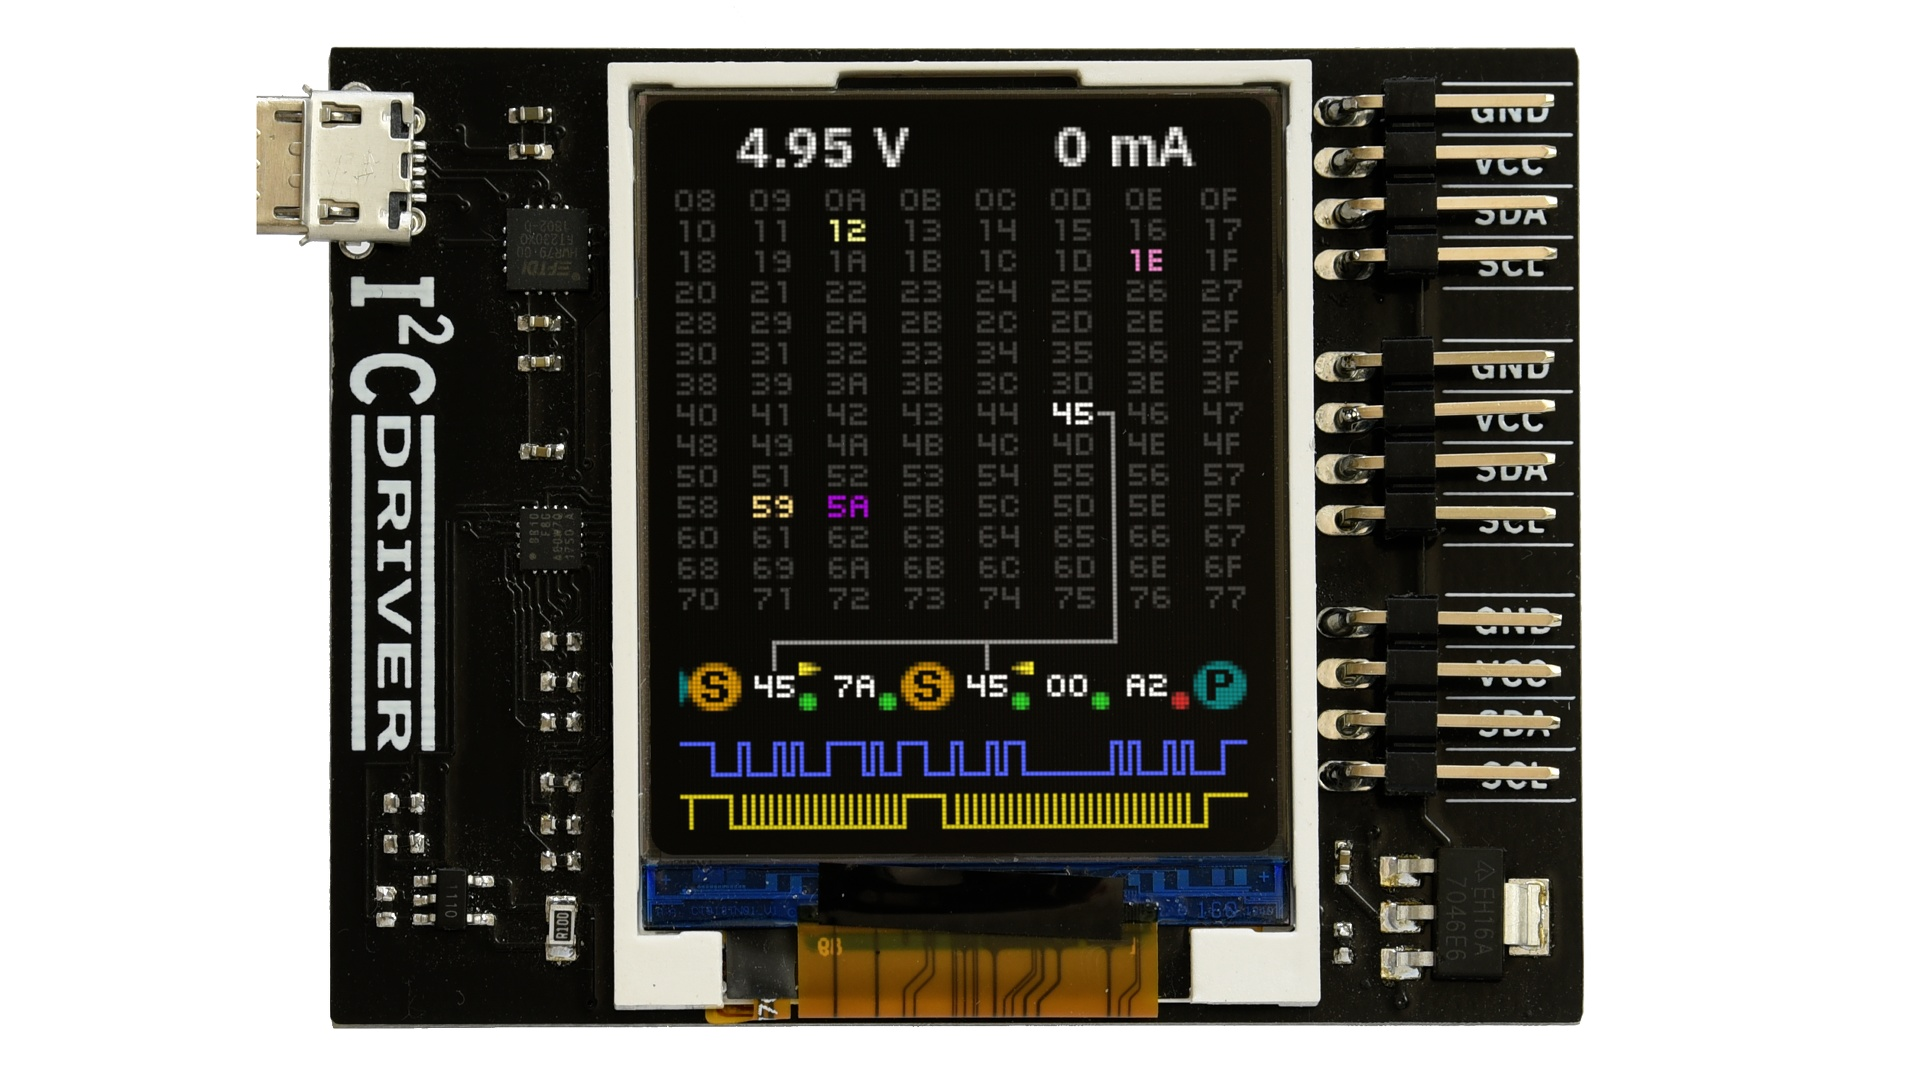
\includegraphics[width=1.00\textwidth]{img/i2cdriver/hero}
\end{center}
\tableofcontents

\newpage

\setlength{\parindent}{0mm}
\setlength{\parskip}{1mm}
\setstretch{1.4}

\section{Overview}

\iicdriver{} is an easy-to-use, open source tool for controlling \iic{} devices. It works with Windows, Mac, and Linux, and has a built-in color screen that shows a live “dashboard” of all the \iic{} activity. It uses a standard FTDI USB serial chip to talk to the PC, so no special drivers need to be installed. The board includes a separate 3.3 V supply with voltage and current monitoring.

\subsection{Features}

\begin{itemize}
\item \textbf{Live display}: shows you exactly what it's doing all the time  
\item \textbf{Supports all \iic{} features}: 7- and 10-bit \iic{} addressing, clock stretching, bus arbitration,
and sustained \iic{} transfers at 400 and 100 kHz  
\item \textbf{\iic{} pullups}: programmable \iic{} pullup resistors, with automatic tuning  
\item \textbf{USB voltage monitoring}: USB line voltage monitor to detect supply problems, to 0.01 V  
\item \textbf{Target power monitoring}: target device high-side current measurement, to 5 mA  
\item \textbf{Three \iic{} ports}: three identical \iic{} ports, each with power and \iic{} signals  
\item \textbf{Jumpers}: three sets of high-quality color coded 100mm jumpers included
\item \textbf{3.3 V output}: output levels are 3.3 V, all are 5 V tolerant  
\item \textbf{Sturdy componentry}: uses an FTDI USB serial adapter, and Silicon Labs automotive-grade EFM8 controller  
\item \textbf{Open hardware}: the design, firmware and all tools are under BSD license
\item \textbf{Flexible control}: GUI, command-line, C/C++, and Python 2/3 host software provided for Windows, Mac, and Linux  
\end{itemize}

\newpage
\section{Getting Started}

When you first connect \iicdriver{} to the USB port, the display blinks white for a moment then shows something like this:

\png{img/i2cdriver/DSC_9039}

Connect the three sets of colored hookup wires as shown,
following the same sequence as on the colored label:

\gap
\begin{center}
\begin{tabular}{ll}
\hline
\mach{GND}  & black \\
\mach{VCC}  & red \\
\mach{SDA}  & blue \\
\mach{SCL}  & yellow \\
\hline
\end{tabular}
\end{center}
\gap

The top two signals carry power, the VCC line supplies 3.3 volts.

Across the top of the display \iicdriver{} continuously measures the USB bus voltage
and the current output.

\newpage
\section{Software installation}

The source for all the \iicdriver{} software is the
\href{https://github.com/jamesbowman/i2cdriver}{repository}.
Available are:

\begin{itemize}
\item a Windows/Mac/Linux GUI
\item a Windows/Mac/Linux command-line
\item Python 2 and 3 bindings
\item Windows/Mac/Linux C/C++ bindings
\end{itemize}

Installation of the GUI and command-line utilities varies by platform.

% Windows
% ^^^^^^^
% 
% This
% `installer <https://github.com/jamesbowman/i2cdriver/releases/download/0.0.04b/i2cdriver-installer.exe>`_
% contains the GUI and command-line utilities.
% 
% The GUI shortcut is installed on the desktop:
% 
% .. im:: images/i2c/win32-icon.png
% 
% launching it brings up the control window:
% 
% .. im:: images/i2c/win32-gui.jpg
% 
% If there is only one serial device, 
% the \iicdriver{} device should be automatically selected.
% If there is more than one device, select its COM port from the pulldown menu at the top.
% Once connected, you can select a connected \iic{} device and write and read data. 
% 
% The command line utility ``i2ccl`` is also installed. For example to display status information::
% 
%   c:\>"c:\Program Files\Excamera Labs\I2CDriver\i2ccl.exe" COM6 i
%   uptime 8991  4.957 V  30 mA  25.8 C SDA=1 SCL=1 speed=100 kHz
% 
% See below for more information on the command-line syntax.
% 
% Linux
% ^^^^^
% 
% ..
%   The Linux GUI is available for download as
%   `i2cgui-linux64 <https://github.com/jamesbowman/i2cdriver/releases/download/v0.1.0/i2cgui-linux64>`_.
%   Or you can run the native Python GUI directly as shown below.
% 
% For the command-line tool, clone the
% `repository <https://github.com/jamesbowman/i2cdriver>`_
% , then do::
% 
%     cd i2cdriver/c
%     make -f linux/Makefile
%     sudo make -f linux/Makefile install
%     i2ccl /dev/ttyUSB0 i
% 
% and you should see something like::
% 
%     uptime 1651  4.971 V  0 mA  21.2 C SDA=1 SCL=1 speed=100 kHz
% 
% MacOS
% ^^^^^
% 
% ..
%   The MacOS GUI is available for download as
%   `i2cgui-macos <https://github.com/jamesbowman/i2cdriver/releases/download/v0.1.0/i2cgui-macos>`_.
%   This is a Mac executable, so after downloading it do::
% 
%       $ cd Downloads
%       $ chmod a+x i2cgui-macos
%       $ ./i2cgui-macos
% 
%   Or you can run the native Python GUI directly as shown below.
% 
% For the command-line tool, clone the
% `repository <https://github.com/jamesbowman/i2cdriver>`_
% , then do::
% 
%     cd i2cdriver/c
%     make -f linux/Makefile
%     sudo make -f linux/Makefile install
%     i2ccl /dev/cu.usbserial-DO00QS8D i
% 
% (substituting your actual \iicdriver{}'s ID for ``DO00QS8D``)
% and you should see something like::
% 
%     uptime 1651  4.971 V  5 mA  21.2 C SDA=1 SCL=1 speed=100 kHz
% 
% Note that the port to use is ``/dev/cu.usbserial-XXXXXXXX``, as explained
% `here <https://pbxbook.com/other/mac-tty.html>`_.
% 
% Python 2 and 3
% ^^^^^^^^^^^^^^
% 
% The \iicdriver{} bindings can be installed with ``pip`` like this::
% 
%     pip install i2cdriver
% 
% then from Python you can read an LM75B temperature sensor with::
% 
%     >>> import i2cdriver
%     >>> i2c = i2cdriver.I2CDriver("/dev/ttyUSB0")   # or something like COM16 for Windows
%     >>> d=i2cdriver.EDS.Temp(i2c)
%     >>> d.read()
%     17.875
%     >>> d.read()
%     18.0
% 
% You can print a bus scan with:
% 
%     >>> i2c.scan()
%     -- -- -- -- -- -- -- -- 
%     -- -- -- -- -- -- -- -- 
%     -- -- -- -- 1C -- -- -- 
%     -- -- -- -- -- -- -- -- 
%     -- -- -- -- -- -- -- -- 
%     -- -- -- -- -- -- -- -- 
%     -- -- -- -- -- -- -- -- 
%     -- -- -- -- -- -- -- -- 
%     48 -- -- -- -- -- -- -- 
%     -- -- -- -- -- -- -- -- 
%     -- -- -- -- -- -- -- -- 
%     -- -- -- -- -- -- -- -- 
%     68 -- -- -- -- -- -- -- 
%     -- -- -- -- -- -- -- -- 
%     [28, 72, 104]
% 
% The Python GUI (which uses `wxPython <https://www.wxpython.org/pages/downloads/>`_) can be run with::
% 
%     python i2cgui.py
% 
% which depending on your distribution looks something like this:
% 
% .. im:: images/i2cdriver-gui-linux.jpg
% 
% There are more examples in the 
% `samples folder in the repository <https://github.com/jamesbowman/i2cdriver/tree/master/python/samples>`_.
% 
% ``help(i2cdriver)`` shows the documentation for the module.
% 
% C/C++
% ^^^^^
% 
% \iicdriver{} is contained in a single source file with a single header.
% Both are in `this subdirectory <https://github.com/jamesbowman/i2cdriver/tree/master/c/common>`_.
% Usage follows the Python API and is fairly self-explanatory.
% 
% The command-line tool ``i2ccl``
% ^^^^^^^^^^^^^^^^^^^^^^^^^^^^^^^
% 
% ``i2ccl`` is the same on all platforms.
% 
% The first parameter to the command is the serial port, which depends on your operating system.
% All following parameters are control commands. These are:
% 
% =================== ==================================================================
%   ``i``             display status information (uptime, voltage, current, temperature)
%   ``d``             device scan
%   ``w`` dev <bytes> write bytes to \iic{} device dev
%   ``p``             send a STOP
%   ``r`` dev N       read N bytes from \iic{} device dev, then STOP
%   ``m``             enter \iic{} bus monitor mode
% =================== ==================================================================
% 
% For example the command::
% 
%   i2ccl /dev/ttyUSB0 r 0x48 2
% 
% reads two bytes from the \iic{} device at address 0x48.
% So with an
% `LM75B temperature sensor <https://www.nxp.com/docs/en/data-sheet/LM75B.pdf>`_
% connected you might see output like::
% 
%   0x16,0x20
% 
% which indicates a temperature of about 22 degrees C.
% 
% \iic{} devices usually have multiple registers.
% To read register 3 of the LM75B, you first write the register address 3, then read two bytes as before::
% 
%   i2ccl /dev/ttyUSB0 w 0x48 3 r 0x48 2
%   0x50,0x00
% 
% Which shows that register 3 has the value ``0x5000``.
% 
% The display
% ===========
% 
% The main display on the screen has three sections.
% The top section is a heat-map showing all 112 legal \iic{} addresses. Devices that are currently active are white. Inactive devices fade to yellow, purple and finally blue.
% The middle section is a symbolic interpretation of current \iic{} traffic. Details on this are below.
% The bottom two lines show a representation of the SDA (blue) and SCL (yellow) signals.
% 
% .. im:: images/i2c/hero2.jpg
% 
% The symolic decode section shows \iic{} transactions as they happen.
% Start and stop are shown as ``S`` and ``P`` symbols.
% After a ``S`` symbol the address byte is shown, with a right arrow (write) or left arrow (read). There are gray lines connecting the address byte to its heat-map indicator.
% Following this is a series of data bytes.
% Each byte is shown in hex, with either a green dot (ACK) or red dot (NACK).
% 
% .. im:: images/i2c/hero3.jpg
% 
% So for example the above sequence is showing
% 
%  * Start, write to address ``45``
%  * Write byte ``7A``
%  * Repeated Start, read from address ``45``
%  * Read byte ``00``
%  * Read byte ``A2``
%  * Stop
% 
% The above sequence is very typical for reading registers from an \iic{} Device.
% Note that the final NACK (red dot) is not an error condition, but the standard way of handling the last byte of read transaction.
% 
% As a monitor
% ============
% 
% In monitor mode, the \iicdriver{} does not write any data to the \iic{} bus.
% Instead it monitors bus traffic and draws it on the display.
% This makes it an ideal tool for troubleshooting and debugging \iic{} hardware and software.
% 
% In monitor mode the mode indicator character in the top-left of the display changes from ``D`` to ``M``.
% 
% There are several ways of entering monitor mode:
% 
% * use the command-line tool::
% 
%     i2ccl m
% 
% * from the GUI check the "Monitor" box
% * from Python issue::
% 
%     i2c.monitor(True)
%   
%   and to exit::
% 
%     i2c.monitor(False)
% 
% * connect a terminal to the \iicdriver{} (at 1000000 8N1) and type the ``m`` character, then type any character to exit monitor mode
% 
% Capture mode
% ============
% 
% Pull-up resistors
% =================
% 
% \iicdriver{} has programmable pull-up resistors.
% 6 control bits each enable or disable a pull-up resistor. These bits are:
% 
% === =============
% Bit Resistor
% === =============
%  0  2.2K to SDA
%  1  4.3K to SDA
%  2  4.7K to SDA
%  3  2.2K to SCL
%  4  4.3K to SCL
%  5  4.7K to SCL
% === =============
% 
% At boot the two 4.7K resistors are enabled.
% By setting combinations of parallel resistors, a range of pull-up strengths can be achieved:
% 
% ==== ==== ==== ====================
% 4.7K 4.3K 2.2K pull-up strength
% ==== ==== ==== ====================
%  0    0     0  0 (i.e. no pull-up)
%  0    0     1  2.2K
%  0    1     0  4.3K
%  0    1     1  1.5K
%  1    0     0  4.7K
%  1    0     1  1.5K
%  1    1     0  2.2K
%  1    1     1  1.1K
% ==== ==== ==== ====================
% 
% Ordering this by useful resistances, the 3-bit combinations are:
% 
% =========== =============
% 3-bit value Resistance
% =========== =============
%   0         0
%   1         2.2K
%   2         4.3K
%   4         4.7K
%   5         1.5K
%   7         1.1K
% =========== =============
% 
% In Python, the pullups are controlled by the ``setpullups()`` method, and the state can be read from the ``pullups`` variable.
% Both are 6-bit values as above.
% 
% The GUI has a control for the pull-up resistors.
% It sets the same pull-up strength for both SDA and SCL.
% 
% Examples
% ========
% 
% The Python ``samples`` directory contains short examples of using all
% `Electric Dollar Store <https://electricdollarstore.com>`_ I2C modules:
% 
% ====== ======================== =================================
% Module Function                 Sample
% ====== ======================== =================================
% DIG2   2-digit 7-seg display    `EDS-DIG2.py    <https://github.com/jamesbowman/i2cdriver/blob/master/python/samples/EDS-DIG2.py>`_
% LED    RGB LED                  `EDS-LED.py     <https://github.com/jamesbowman/i2cdriver/blob/master/python/samples/EDS-LED.py>`_
% POT    potentiometer            `EDS-POT.py     <https://github.com/jamesbowman/i2cdriver/blob/master/python/samples/EDS-POT.py>`_
% BEEP   Piezo beeper             `EDS-BEEP.py    <https://github.com/jamesbowman/i2cdriver/blob/master/python/samples/EDS-BEEP.py>`_
% REMOTE IR remote receiver       `EDS-REMOTE.py  <https://github.com/jamesbowman/i2cdriver/blob/master/python/samples/EDS-REMOTE.py>`_
% EPROM  CAT24C512 64 Kbyte EPROM `EDS-EPROM.py   <https://github.com/jamesbowman/i2cdriver/blob/master/python/samples/EDS-EPROM.py>`_
% MAGNET LIS3MDL magnetometer     `EDS-MAGNET.py  <https://github.com/jamesbowman/i2cdriver/blob/master/python/samples/EDS-MAGNET.py>`_
% TEMP   LM75B temperature sensor `EDS-TEMP.py    <https://github.com/jamesbowman/i2cdriver/blob/master/python/samples/EDS-TEMP.py>`_
% ACCEL  RT3000C Accelerometer    `EDS-ACCEL.py   <https://github.com/jamesbowman/i2cdriver/blob/master/python/samples/EDS-ACCEL.py>`_
% CLOCK  HT1382 real-time clock   `EDS-CLOCK.py   <https://github.com/jamesbowman/i2cdriver/blob/master/python/samples/EDS-CLOCK.py>`_
% ====== ======================== =================================
% 
% All demos and applications are run the same way, supplying the \iicdriver{} on the command-line. For example::
% 
%     python EDS-LED.py COM16
% 
% Also included are some small applications which demonstrate combinations of modules:
% 
% Color Compass
% ^^^^^^^^^^^^^
% 
% Source code: `EDS-color-compass.py <https://github.com/jamesbowman/i2cdriver/blob/master/python/samples/EDS-color-compass.py>`_
% 
% Color compass uses MAGNET and LED, reading the current magnetic field direction and rendering it as a color on the LED.
% As you twist the module, the color changes.
% For example there is a particular direction for pure red, as well as all other colors.
% The code
% reads the magnetic field direction, scales the values to 0-255, and sets the LED color.
% 
% Egg Timer
% ^^^^^^^^^
% 
% Source code: `EDS-egg-timer.py <https://github.com/jamesbowman/i2cdriver/blob/master/python/samples/EDS-egg-timer.py>`_
% 
% The demo uses POT, DIG2 and BEEPER to make a simple kitchen egg timer.
% Twisting the POT sets a countdown time in seconds,
% and after it's released the ticker starts counting.
% When it reaches "00" it flashes and beeps.
% 
% Take-a-ticket
% ^^^^^^^^^^^^^
% 
% Source code: `EDS-take-a-ticket.py <https://github.com/jamesbowman/i2cdriver/blob/master/python/samples/EDS-take-a-ticket.py>`_
% 
% This demo runs a take-a-ticket display for a store or deli counter,
% using REMOTE, DIG2 and BEEP modules.
% It shows 2-digit "now serving" number, and each time '+' is
% pressed on the remote it increments the counter and
% makes a beep, so the next customer can be served.
% Pressing '-' turns the number back one.
\newpage
\section{Technical notes}

\subsection{Port names}

The serial port that \iicdriver{} appears at depends on your operating system.

On \textbf{Windows}, it appears as COM1, COM2, COM3 etc.
You can use the Device Manager or the \mach{MODE} command to display the available ports.
\href{https://plugable.com/2011/07/04/how-to-change-the-com-port-for-a-usb-serial-adapter-on-windows-7/}{This article}
describes how to set a device to a fixed port.

On \textbf{Linux}, it appears as \mach{/dev/ttyUSB0}, 1, 2 etc.
The actual number depends on the order that devices were added.
However it also appears as something like:
\begin{lstlisting}
    /dev/serial/by-id/usb-FTDI_FT230X_Basic_UART_DO00QS8D-if00-port0
\end{lstlisting}
Where \mach{DO00QS8D} is the serial code of the \iicdriver{} (which is printed on the bottom of each \iicdriver{}).
This is longer, of course, but always the same for a given device.

Similarly on \textbf{Mac OS}, the \iicdriver{} appears as \mach{/dev/cu.usbserial-DO00QS8D}.

\subsection{Decreasing the USB latency timer}

\iicdriver{} performance can be increased by setting the USB latency timer to its minimum value of 1 ms.
This can increase the speed of two-way \iic{} traffic by up to 10X.

On \textbf{Linux} do:

\begin{lstlisting}
    setserial /dev/ttyUSB0 low_latency
\end{lstlisting}

On \textbf{Windows} and \textbf{Mac OS} follow
\href{https://projectgus.com/2011/10/notes-on-ftdi-latency-with-arduino/}{these instructions}.

\subsection{Temperature sensor}

The temperature sensor is located in the on-board EFM8 microcontroller.
It is calibrated at manufacture to within 2 C.
A sudden temperature rise may indicate that one of the output pins (MOSI, SCK, CS, A, or B) is shorted to VCC or GND.

\subsection{Raw protocol}

\iicdriver{} uses a serial protocol to send and receive \iic{} commands.
Connect to the \iicdriver{} at 460800 baud, 8 bits, no parity, 1 stop bit (460800 8N1).
Many \iicdriver{} commands are ASCII, you can control it
interactively from any terminal application that can connect at 460800
baud. For example typing u and s toggles the CS line and ? displays the
status info.
Commands are:

\gap\begin{tabular}{ll}
\hline
\mach{?}        & transmit status information (see below)        \\
\mach{e} $byte$ & echo $byte$       \\
\mach{s}        & select        \\
\mach{u}        & unselect        \\
\mach{a} $byte$ & set A output to 0/1       \\
\mach{b} $byte$ & set B output to 0/1       \\
\mach{x}        & disconnect from SPI bus       \\
\mach{0x80-bf}  & write and read 1-64 bytes       \\
\mach{0xc0-ff}  & write 1-64 bytes        \\ \hline
\end{tabular}\gap

So for example to select, transfer two bytes
\mach{0x12,0x34},
unselect, the host sends 5 bytes.
The command \mach{0x81} is a two byte send/receive, so two bytes are returned to the PC.

\begin{lstlisting}
s
0x81
0x12
0x34
u
\end{lstlisting}


The status information is always 80 characters, space padded. For example:

{\scriptsize
\begin{framed}\begin{Verbatim}
[spidriver1 DO00QS8D 000007219 4.807 045 25.4 1 1 1 49c1                       ]
\end{Verbatim}
\end{framed}}

The fields are space-delimited:

\gap\begin{tabular}{ll}
\hline
spidriver1      & fixed identifier \\
serial          & serial code identifier \\
uptime          & \iicdriver{} uptime 0-999999999, in seconds \\
voltage         & USB bus voltage, in volts \\
current         & attached device current, in mA \\
temperature     & junction temperature, in C \\
CS              & CS line state \\
A               & A line state \\
B               & B line state \\
crc             & 16-bit CRC of all input and output bytes (CRC-16-CCITT) \\
\hline
\end{tabular}\gap

\newpage
\hypertarget{technical-specifications}{}
\hypertarget{technical-specifications}{%
\subsection{Specifications}\label{electrical-characteristics}}

\subsubsection*{DC characteristics}
\vspace{10 pt}
{\renewcommand{\arraystretch}{1.2}% for the vertical padding

\begin{tabularx}{\linewidth}{XC{40pt}C{40pt}C{40pt}C{40pt}}
\heavyline
& min & typ & max & units \\ \heavyline

Voltage accuracy              && 0.01 && V            \\ \hline
Current accuracy              && 5 && mA              \\ \hline
Temperature accuracy          && $\pm$ 2 && $^{\circ}$C            \\ \hline
SDA,SCL & & & & \\
\hspace{10pt}low voltage & & & 0.6 & V \\
\hspace{10pt}high voltage & 2.7 &   & 5.8 & V \\ \hline
Output current        & & & 470 & mA                  \\ \hline
Current consumption   & & 25 & & mA                   \\ \hline

\end{tabularx}}
\vspace{10 pt}

\subsubsection*{AC characteristics}
\vspace{10 pt}

{\renewcommand{\arraystretch}{1.2}% for the vertical padding
\begin{tabularx}{\linewidth}{XC{40pt}C{40pt}C{40pt}C{40pt}}
\heavyline
& min & typ & max & units \\ \heavyline

\iic{} speed                     &100& &400& Kbps   \\ \hline
Uptime accuracy               && 150 && ppm           \\ \hline
Uptime rollover               && 31.7 && years        \\ \hline
Startup time & & & 200 & ms \\ \hline
\end{tabularx}}
\vspace{10 pt}

\section{Support information}

Technical and product support is available at
\href{mailto:support@i2cdriver.com}{support@i2cdriver.com}

\iicdriver{} is built and maintained by
\href{https://excamera.com}{Excamera Labs}.


\end{document}
